\graphicspath{{../../S28_Proprietes_des_symetries/Images/}}

\themeM
\chapter{Propriétés des symétries}
\label{S28}

\textcolor{teal}{\bf Compétences :}
   \begin{competences}
      \item Comprendre l’effet d’une symétrie (axiale et centrale) sur une figure.
      \item Mobiliser les connaissances des transformations au programme pour déterminer des grandeurs géométriques.
      \item Mener des raisonnements et s’initier à la démonstration en utilisant des transformations.
   \end{competences}

\vfill

\begin{debat}{Débat : les mandalas}
   {\bf Mandala} est un terme sanskrit qui signifie {\it cercle}. Il désigne plus largement un objet support à la méditation et à la concentration composé de cercles; de symétries et de formes diverses.
   \tcblower
      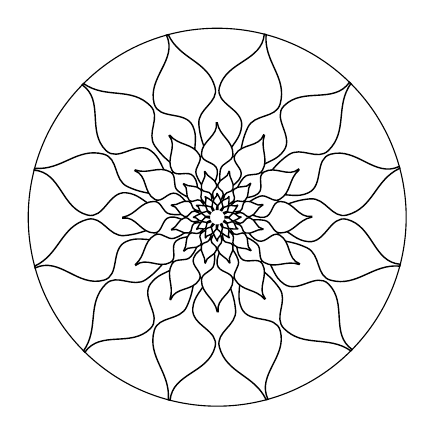
\begin{tikzpicture}[scale=0.2,pics/leaf/.style={code={\pgfgettransformentries{\myxx}{\myxy}{\myyx}{\myyy}{\tmp}{\tmp}\pgfmathsetmacro{\myscale}{sqrt(\myxx*\myyy-\myxy*\myyx)} \draw[line width=0.5,pic actions] (-0.02,0) to[out=80,in=-80] (0,0.1) to[out=100,in=-90] (-0.1,0.2) to[out=90,in=-80] (-0.006,0.4) -- (0,0.4) to[out=-80,in=90] (0.1,0.2) to[out=-90,in=80] (0.02,0.1) to[out=-100,in=95] (0.02,0) -- cycle;}}]
         \path foreach \Radius [count=\Cnt] in {4,2,1,0.5} {foreach \Angle [evaluate=\Angle as \EffAngle using {\Angle-15*\Cnt}] in {0,30,...,330} { (\EffAngle:\Radius) pic[rotate=\EffAngle-90,scale=\Radius,fill=white]{leaf}}};
         \draw (0,0) circle (12) ;
      \end{tikzpicture}
\end{debat}

\hfill {\gray Vidéo : \href{https://www.youtube.com/watch?time_continue=262&v=bgoHUH-_yWo&feature=emb_logo}{\bf Tibet sand painting of Mandala}, chaîne YouTube {\it Tibet travel}.}


%%% Approche %%%
\begin{Maquette}[Cours]{Theme={Activité d'approche},Couleur={SteelBlue}}

   \AAtitre{Propriétés des symétries}

      {\it Objectifs : observer l'effet d'une symétrie centrale ou d'une symétrie axiale sur les longueurs, les angles, le parallélisme et l'alignement ; utiliser un logiciel de géométrie dynamique.}

      \begin{AActivite}

         Ouvrir Geogebra et choisir l'onglet \textbf{Géométrie}.

         \AApartie{Symétrie axiale}
            \begin{center}
               {\hautab{0.8}
               \begin{tabular}{|c|p{6cm}|p{2.6cm}|>{\itshape\footnotesize}p{5cm}|}
                  \hline
                  1 & \multicolumn{3}{l|}{Construction de la {\bf figure} et de l'{\bf axe de symétrie}} \\
                  & Tracer un quadrilatère $ABCD$ & polygone & cliquer en quatre points du plan \\
                  & Placer un point $E$ sur la droite $(AB)$ & point sur objet & cliquer quelque part sur la droite $(AB)$ \\
                  & Tracer la parallèle à $(BC)$ passant par $D$ & parallèle & cliquer sur le segment $[BC]$ puis sur $D$ \\
                  & Tracer une droite $(FG)$ & droite & cliquer en deux points du plan \\
                  \hline
                  2 & \multicolumn{3}{l|}{Construction de la figure {\bf symétrique par rapport à l'axe} $(FG)$} \\
                  & Tracer la figure symétrique & symétrie axiale & sélectionner successivement chaque élément de la figure, puis la droite $(FG)$ \\
                  \hline
                  3 & \multicolumn{3}{l|}{Faire apparaître différentes {\bf mesures}} \\
                  & Mesurer la longueur du segment $[AD]$ & distance & cliquer sur le segment $[AD]$ \\
                  & Mesurer l'angle $\widehat{ABC}$ & angle & cliquer sur les trois points de l'angle \\
                  \hline
               \end{tabular}}
            \end{center}
            \begin{enumerate}
               \item Observer ce qu'il se passe lorsque l'on déplace un point du quadrilatère $ABCD$ ou de l'axe de symétrie.
               \item Comparer la longueur du segment $[AD]$ et celle du segment $[A'D']$ : \pointilles
               \item Comparer la mesure de l'angle $\widehat{ABC}$ et celle de l'angle $\widehat{A'B'C'}$ : \pointilles
               \item Où se situe le point $E'$ ? \pointilles
               \item Les deux droites parallèles entre elles dans la figure d'origine le restent-elles dans la figure symétrique ? \pointilles
            \end{enumerate}

         \AApartie{Symétrie centrale}
            \begin{center}
               {\hautab{0.8}
               \begin{tabular}{|c|p{6cm}|p{2.6cm}|>{\itshape\footnotesize}p{5cm}|}
                  \hline
                  1 & \multicolumn{3}{l|}{Construction de la {\bf figure} et du {\bf centre de symétrie}} \\
                  & Tracer un pentagone $ABCDE$ & polygone & cliquer en cinq points du plan \\
                  & Placer un point $F$ sur la droite $(AB)$ & point sur objet & cliquer quelque part sur la droite $(AB)$ \\
                  & Tracer la parallèle à $(CD)$ passant par $E$ & parallèle & cliquer sur le segment $[CD]$ puis sur $E$ \\
                  & Placer un point $(G)$ & point & cliquer en un point du plan \\
               \hline
                  2 & \multicolumn{3}{l|}{Construction de la figure {\bf symétrique par rapport au centre} $G$} \\
                  & Tracer la figure symétrique & symétrie centrale & sélectionner successivement chaque élément de la figure, puis le point $G$ \\
                  \hline
                  3 & \multicolumn{3}{l|}{Faire apparaître différentes {\bf mesures}} \\
                  & Mesurer la longueur du segment $[BC]$ & distance & cliquer sur le segment $[BC]$ \\
                  & Mesurer l'angle $\widehat{CDE}$ & angle & cliquer sur les trois points de l'angle \\
               \hline
               \end{tabular}}
            \end{center}
            \begin{enumerate}[resume]
               \item Observer ce qu'il se passe lorsque l'on déplace un point du pentagone $ABCDE$ ou le point $G$.
               \item Comparer la longueur du segment $[BC]$ et celle du segment $[B'C']$ : \pointilles
               \item Comparer la mesure de l'angle $\widehat{CDE}$ et celle de l'angle $\widehat{C'D'E'}$ : \pointilles
               \item Où se situe le point $F'$ ? \pointilles
               \item Les deux droites parallèles entre elles dans la figure d'origine restent-elles parallèles dans la figure symétrique ? \pointilles
         \end{enumerate}

      \end{AActivite}

\end{Maquette}


%%%Trace écrite %%%
\begin{Maquette}[Cours]{Theme={Trace écrite},Couleur={0.4[SteelBlue,Black]}}

   %%%1
   \section{Rappels sur les symétries}

      \begin{definition*}{}
         \begin{itemize}
            \item $M'$ est l'image du point $M$ par la \textbf{symétrie d'axe $\Delta$} signifie que la droite $\Delta$ est la médiatrice du segment $[MM']$.
            \item $M'$ est l'image du point $M$ par la \textbf{symétrie de centre $O$} signifie que $O$ est le milieu du segment $[MM']$.
         \end{itemize}
      \end{definition*}
         
      \begin{center}
         {\psset{unit=0.9}
         \begin{pspicture}(-4,-1)(4,4)
            \pstGeonode[PointName=none, PointSymbol=none](0,-0.5){O}(0,3.5){O'}
            \pstLineAB{O}{O'}
            \pstTriangle[PosAngleA=115](1,1){A}(4,0){B}(2,3){C}
            \psset{CodeFig=true,CodeFigColor=DodgerBlue,linecolor=Crimson,RightAngleSize=0.2}
            \pstOrtSym[SegmentSymbol=pstslash, PosAngle=50]{O}{O'}{A}
            \pstOrtSym[SegmentSymbol=pstslashh,PosAngle=-135]{O}{O'}{B}
            \pstOrtSym[SegmentSymbol=pstslashhh,PosAngle=90]{O}{O'}{C}
            \pstLineAB[linecolor=Crimson]{A'}{B'}
            \pstLineAB[linecolor=Crimson]{B'}{C'}
            \pstLineAB[linecolor=Crimson]{C'}{A'}
            \rput(0,3.8){$\Delta$}
         \end{pspicture}
         \quad
         \begin{pspicture}(-5,-1)(4,3)
            \pstGeonode[PosAngle=-90](0,1.5){O}
            \pstTriangle(1,0){A}(4,0){B}(2,2){C}
            \pstSymO[CodeFig=true,CodeFigColor=DodgerBlue,PosAngle={40,170,-90}]{O}{A, B, C}[A', B', C']
            \pstLineAB[linecolor=Crimson]{A'}{B'}
            \pstLineAB[linecolor=Crimson]{C'}{B'}
            \pstLineAB[linecolor=Crimson]{A'}{C'}
         \end{pspicture}}
      \end{center}


%%%2
\section{Propriétés des symétries}
  
   \begin{propriete*}{}
      La symétrie axiale et la symétrie centrale {\bf conservent} les longueurs, les angles, l'alignement et le parallélisme (ce sont des isométries).
   \end{propriete*}

   \begin{exemple*}{}
      On considère la figure $A'B'C'D'$ symétrique de $ABCD$ par rapport au point $O$ et la figure $A''B''C''D''$ symétrique de $ABCD$ par rapport à la droite $(d)$. \par
      \begin{minipage}{9.5cm}
         {\psset{unit=0.8} \small
         \begin{pspicture}(-5,-7)(6,6)
            \pstGeonode[PosAngle=-90](0.5,2){O}
            \pstGeonode[PointName=none,PointSymbol=none](-3,-5){N}(3,1){P}
            \pstLineAB{N}{P}
            \pstGeonode[PosAngle={-45,-90,-135,135,45},CurveType=polygon,PointSymbol=+](0,0){A}(-2,0){I}(-4,0){B}(-4,2){C}(-2,2){D}
            \pstSymO[PosAngle={135,90,45,-45,-135},CurveType=polygon,PointSymbol=+,linecolor=Crimson]{O}{A,I,B,C,D}[A',I',B',C',D']
            \pstOrtSym[PosAngle={90,180,-135,-45,45},CurveType=polygon,PointSymbol=+,linecolor=DodgerBlue]{N}{P}{A,I,B,C,D}[A'',I'',B'',C'',D'']
            \pstRightAngle{B}{C}{D}
            \pstRightAngle[linecolor=Crimson]{B'}{C'}{D'}
            \pstRightAngle[linecolor=DodgerBlue]{B''}{C''}{D''}
            \rput(3,0.2){$(d)$}
         \end{pspicture}}
      \end{minipage}
      \quad 
      \begin{minipage}{6.5cm}
         Propriétés conservées : \par
         \begin{itemize}
            \item L'alignement : \par
               $I\in[AB]$ donc : $\Syst{I'\in[A'B']}{I''\in[A''B'']}$ \par
            \item le parallélisme : \par
               $(AB)//(CD)$ donc : $\Syst{(A'B')//(C'D')}{(A''B'')//(C''D'')}$ \par
            \item Les longueurs : \par
               $A'B' = AB$ et $A''B'' = AB$ \par
               $IA=IB$ donc $\Syst{I'A'=I'B'}{I''A''=I''B''}$ \par
            \item Les angles : \par
               $(BC)\perp(CD)$ donc $\Syst{(B'C')\perp(C'D')}{(B''C'')\perp(C''D'')}$
         \end{itemize}
      \end{minipage}
   \end{exemple*}

\end{Maquette}


%%% Exercices %%%
\begin{Maquette}[Fiche,CorrigeFin,Colonnes=2]{}

   \begin{exercice}[SLF] %1
      Pour chacune des figures suivantes, dire s'il s'agit ou pas d'une symétrie (axiale ou centrale). Si oui, tracer l'axe ou le centre de symétrie.
      \begin{center}
         {\psset{unit=1}
         \begin{pspicture}(15,6.3)
            \psframe(0,0)(15,6)
            \psline(5,0)(5,6)
            \psline(10,0)(10,6)
            \psline(0,3)(15,3)
            \rput(0.5,5.5){a.}
            \rput(1.5,4.5){\cocottea}
            \rput(4.5,4.5){\cocottec}
            \rput(5.5,5.5){b.}
            \rput(7.5,4.75){\cocotteb}
            \rput{180}(7.5,4.25){\cocottea} 
            \rput(10.5,5.5){c.}
            \rput(11.5,4.75){\cocottea}
            \rput(11.5,3.25){\cocotteb}
            \rput(0.5,2.5){d.}
            \rput{90}(2,1){\cocotteb}
            \rput(2,1){\cocottea} 
            \rput(5.5,2.5){e.}
            \rput(6.25,1.5){\cocottea}
            \rput(9,1){\cocottec}
            \rput(10.5,2.5){f.}
            \rput{-30}(10.5,1){\cocottea}
            \rput{80}(14.5,2.5){\cocottec}
         \end{pspicture}}
      \end{center}
   \end{exercice}

   \begin{multicols}{2}
      
      \begin{Solution}
         {\psset{unit=0.85} \small
            \begin{pspicture}(0.3,3)(5,6.2)
               \psframe(0,3)(5,6)
               \rput(0.5,5.5){a.}
               \rput(1.5,4.5){\cocottea}
               \rput(4.5,4.5){\cocottec}
               \psline[linecolor=RoyalBlue](3,3.25)(3,5.75)
               \rput(3.4,3.5){\cor{$d$}}
               \rput(1.4,3.25){\cor{symétrie d'axe $d$}}
            \end{pspicture}
            \begin{pspicture}(5,3)(10,5.5)
               \psframe(5,3)(10,6)
               \rput(5.5,5.5){b.}
               \rput(7.5,4.75){\cocotteb}
               \rput{180}(7.5,4.25){\cocottea} 
               \psdot[linecolor=RoyalBlue](7.5,4.5)
               \rput(7.8,4.5){\cor{o}}
               \rput(9,3.6){\cor{symétrie de}}
               \rput(9,3.25){\cor{centre o}}
            \end{pspicture} \par
            \begin{pspicture}(8,0)(15,3)
                  \psframe(10,0)(15,3)
                  \rput(10.5,2.5){f.}
                  \rput{-30}(10.5,1){\cocottea}
                  \rput{80}(14.5,2.5){\cocottec}
                  \psline[linecolor=RoyalBlue](12.9,0.4)(12.3,2.8)
                  \rput(12.5,2.6){\cor{$\Delta$}}
                  \rput(13.5,0.25){\cor{symétrie d'axe $\Delta$}}
            \end{pspicture}}
      \end{Solution}


      \begin{exercice}[Dur] %2
         Soit $ABC$ un triangle isocèle en $A$ tel que \par
         $BC=\Lg{3}$ et $BA=\Lg{4}$.
         \begin{enumerate}
            \item Construire le triangle $ABC$.
            \item Construire le symétrique de $ABC$ par apport à $A$ \par
               ($D$ est le symétrique de $B$ et $E$ celui de $C$).
            \item Construire le milieu $I$ de $[BC]$ et $J$ celui de $[DE]$.
            \item Démontrer que les trois points $J, A$ et $I$ sont alignés. Que représente la droite $(IJ)$ pour les segments $[BC]$ et $[DE]$ ?
         \end{enumerate}
      \end{exercice}
      
      \begin{Solution}
         \begin{pspicture}(-0.5,-0.3)(7.5,3.5)
            \psset{PointSymbol=none}
            \pstGeonode[PosAngle={-135,135,90,180,0}]{B}(0,3){C}(3.71,1.5){A}(0,1.5){I}(7.42,1.5){J}
            \pstLineAB{B}{C}
            \pstSymO[PosAngle={45,-135}]{A}{B,C}[D,E]
            \pstSegmentMark{A}{B}
            \pstSegmentMark{A}{C}
            \pstLabelAB[offset=-3mm]{B}{C}{\Lg{3}}
            \pstLabelAB{B}{A}{\Lg{4}}
            \pstSegmentMark[SegmentSymbol=pstslash]{B}{I}
            \pstSegmentMark[SegmentSymbol=pstslash]{C}{I}
            \pstSegmentMark[SegmentSymbol=pstslash]{E}{J}
            \pstSegmentMark[SegmentSymbol=pstslash]{D}{J}
            \psset{linecolor=Crimson}
            \pstSegmentMark{A}{D}
            \pstSegmentMark{A}{E}
            \pstLineAB{E}{D}
            \pstLineAB[linecolor=RoyalBlue]{I}{J}
         \end{pspicture} \par
         \begin{itemize}
            \item Le triangle $ABC$ est isocèle en $A$ et $I$ est le milieu de $[BC]$ donc, la droite $(AI)$ est la hauteur issue de $A$ dans le triangle $ABC$, mais aussi la médiatrice du segment $[BC]$. On a alors $(AI) \perp (BC)$. \smallskip
            \item Le triangle $ADE$ est le symétrique du triangle $ABC$ par la symétrie centrale de centre $A$, par conservation des angles, on a $(AJ)\perp(DE)$. \smallskip
            \item De plus, la droite $(BC)$ est transformée en la droite $(DE)$ qui lui est parallèle donc, on a $\left.\begin{array}{c} (AI) \perp (BC)\,\\\,(AJ)\perp(DE) \\ (BC) // (DE) \end{array}\right\}$ soit $(AI) // (AJ)$. \smallskip
            \item Par conséquent, \cor{les points $J$, $A$ et $I$ sont alignés.}
            \item La droite $(IJ)$ est la \cor{médiatrice} des segments $[BC]$ et $[DE]$.
         \end{itemize}
      \end{Solution}
      

      \begin{exercice} %3
         Le dessin ci-dessous n'est pas à taille réelle. Les points $D, O$ et $A$ sont alignés.
         \begin{center}
            {\psset{unit=0.9} \small
            \begin{pspicture}(-4,-0.5)(4,3.5)
               \pstGeonode[PosAngle={-90,-90,-45,45,-90},PointSymbol=+](-4,0){D}(3.5,0){A}(3.5;30){B}(3;120){C}(0,0){O}
               \pstLineAB[nodesepB=-1]{D}{A}
               \pstLineAB[nodesepB=-0.5]{O}{C}
               \pstLineAB[nodesepB=-1]{O}{B}
               \pstMarkAngle[MarkAngleRadius=0.7]{C}{O}{D}{\ang{60}}
               \pstMarkAngle[MarkAngleRadius=1,MarkAngleType=double,LabelSep=1.6]{A}{O}{B}{\ang{30}}
               \pstLabelAB{O}{B}{\Lg{6}}
               \pstLabelAB{C}{O}{\Lg{4}}
               \pstLabelAB[offset=-3mm]{D}{O}{\Lg{3}}
               \pstLabelAB[offset=-3mm]{O}{A}{\Lg{5}}
            \end{pspicture}}
         \end{center}
         \begin{enumerate}
            \item Reproduire en vraie grandeur ce dessin.
            \item Construire les points $E$ et $F$, symétriques respectifs de $B$ et $C$ par rapport à $O$. \par
               Julie affirme que l'angle $\widehat{BOF}$ mesure \ang{60} et l'angle $\widehat{COE}$ mesure \ang{90}. À-t-elle raison ? Si oui, justifier ; sinon, corriger son affirmation.
         \end{enumerate}
      \end{exercice}
      
      \begin{Solution}
         Figure à l'échelle 3/4. \par
         {\psset{unit=0.75} \small
         \begin{pspicture}(-5.5,-4)(6,4.1)
            \pstGeonode[PosAngle={-90,-90,-45,45,-90},PointSymbol=+](-3,0){D}(5,0){A}(6;30){B}(4;120){C}(0,0){O}(4;-60){F}(6;-150){E}
            \pstLineAB{D}{A}
            \pstMarkAngle[MarkAngleRadius=0.7]{C}{O}{D}{\ang{60}}
            \pstMarkAngle[MarkAngleRadius=1,MarkAngleType=double,LabelSep=1.6]{A}{O}{B}{\ang{30}}
            \pstLabelAB{O}{B}{\Lg{6}}
            \pstLabelAB{C}{O}{\Lg{4}}
            \pstLabelAB[offset=-3mm]{D}{O}{\Lg{3}}
            \pstLabelAB[offset=-3mm]{O}{A}{\Lg{5}}
            \pstSegmentMark{O}{B}
            \pstSegmentMark[linecolor=RoyalBlue]{O}{E}
            \pstSegmentMark[SegmentSymbol=pstslash]{O}{C}
            \pstSegmentMark[SegmentSymbol=pstslash,linecolor=RoyalBlue,CodeFigColor=RoyalBlue]{O}{F}
         \end{pspicture}}
         \begin{itemize}
            \item \cor{Julie a tort pour l'angle $\widehat{BOF}$} : on a $\widehat{BOF} =\widehat{BOA}+\widehat{AOF}$. \par
               Par conservation des angles par symétrie centrale, \par
               on a $\widehat{AOF} =\widehat{DOC} =\ang{60}$ donc, \par
               $\widehat{BOF} =\ang{30}+\ang{60} =\ang{90}$. \cor{L'angle $\widehat{BOF}$ est droit}.
            \item \cor{Julie a raison pour l'angle $\widehat{COE}$} : on a $\widehat{COE} =\widehat{COD}+\widehat{DOE}$. \par
               Par conservation des angles par symétrie centrale, \par
               on a $\widehat{DOE} =\widehat{AOB} =\ang{30}$ donc, $\widehat{COE} =\ang{60}+\ang{30} =\ang{90}$.
         \end{itemize}
      \end{Solution}
      

      \begin{exercice} %4
         Programme de construction :
         \begin{itemize}
            \item Tracer un triangle $MOP$ tel que: $OM =\Lg{2,5}$ ; $OP =\Lg{3}$ et $\widehat{POM} =\ang{70}$.
            \item Tracer la droite $(d)$ perpendiculaire à la droite $(OP)$ passant par le point $P$.
            \item Tracer le symétrique du triangle $MOP$ par rapport à la droite $(d)$ : on notera $M'$ le symétrique de $M$ par rapport à la droite $(d)$, $O'$ celui de $O$.
         \end{itemize}
         \begin{enumerate}
            \item Quelle devrait-être la mesure de $PO'$ ? Vérifier.
            \item Quelle devrait-être la mesure de $M'O'$ ? Vérifier.
            \item Quelle devrait-être la mesure de $\widehat{PO'M'}$ ? Vérifier.
          \end{enumerate}
      \end{exercice}
      
      \begin{Solution}
         \begin{pspicture}(-1,-0.5)(6,3.2)
            \psset{PointSymbol=none}
            \pstTriangle{O}(3,0){P}(2.5;70){M}
            \pstGeonode(3,2.5){d}
            \pstLineAB[nodesep=-0.5,linecolor=DodgerBlue]{P}{d}
            \pstOrtSym[CurveType=polygon,linecolor=Crimson,PosAngle={-100,90,-5}]{P}{d}{O,M,P}[O',M',P]
            \pstLabelAB[offset=-3mm]{O}{P}{\Lg{3}}
            \pstLabelAB{O}{M}{\Lg{2,5}}
            \pstMarkAngle{P}{O}{M}{\ang{70}}
         \end{pspicture}
         \begin{enumerate}
            \item Par conservation des longueurs : $PO' =PO =\cor{\Lg{3}}$.
            \item Par conservation des longueurs : $M'O' =MO =\cor{\Lg{2,5}}$.
            \item Par conservation des angles : $\widehat{PO'M'} =\widehat{POM} =\cor{\ang{70}}$.
         \end{enumerate}
      \end{Solution}

      
      \begin{exercice}[Dur] %5
         Un quadrilatère $ABCD$ est appelé isocerfvolant en $A$ si l'angle $\widehat{BAD}$ est droit et si la droite $(AC)$ est un axe de symétrie.
         \begin{enumerate}
            \item
               \begin{enumerate}
                  \item Construire un quadrilatère ABCD qui soit un isocerfvolant en A.
                  \item Construire un quadrilatère qui admette un axe de symétrie et qui ne soit pas un isocerfvolant.
               \end{enumerate}
            \item
               \begin{enumerate}
                  \item Dans un isocerfvolant, montrer que $\widehat{DAC} =\widehat{BAC}$
                  \item En déduire la mesure de l'angle $\widehat{DAC}$
                  \item Quelle est la position relative de $(BD)$ et $(AC)$ ?
               \end{enumerate}
            \item Les affirmations suivantes sont-elles vraies ou fausses ? Justifier les réponses.
            
         \end{enumerate}
      \end{exercice}
      
      \begin{Solution}
         \begin{enumerate}
            \item 
               \begin{enumerate}
                  \item Quadrilatère $ABCD$ isocerfvolant en $A$ : \par
                     \begin{pspicture}(-1.5,-1.5)(6,1.7)
                        \pstGeonode[PointSymbol=none,CurveType=polygon,PosAngle={135,-90,45,90}]{A}(1,-1){B}(4,0){C}(1,1){D}
                        \pstLineAB[linecolor=RoyalBlue,nodesep=-1]{A}{C}
                        \pstRightAngle[linecolor=Crimson]{D}{A}{B}
                     \end{pspicture}
                  \item Quadrilatère $ABCD$ non isocervolant ayant un axe de symétrie : \par
                     \begin{pspicture}(-2,-2.5)(6,2)
                        \pstGeonode[PointSymbol=none,CurveType=polygon,PosAngle={135,-90,45,90}]{A}(1,-2){B}(4,0){C}(1,2){D}
                        \pstLineAB[linecolor=RoyalBlue,nodesep=-1]{A}{C}
                     \end{pspicture}
               \end{enumerate}
            \item 
               \begin{enumerate}     
                  \item $(AC)$ est un axe de symétrie de la figure $ABCD$, donc par conservation des angles, $\cor{\widehat{DAC} =\widehat{BAC}}$.
                  \item $\widehat{DAB} =\ang{90}$, donc $\widehat{DAC}$ vaut la moitié, c'est-à-dire $\cor{\ang{45}}$.
                  \item $B$ est le symétrique de $D$ par rapport à $(AC)$ donc, \cor{les droites $(BD)$ et $(AC)$ sont perpendiculaires}.
               \end{enumerate}
            \item
               \begin{enumerate}
                  \item \cor{Un carré est un isocervolant} car ses diagonales sont des axes de symétrie et tous ses angles mesurent \ang{90}.
                  \item \cor{Un rectangle n'est pas un isocervolant} car ses diagonales ne sont pas des axes de symétrie.
               \end{enumerate}
         \end{enumerate}
      \end{Solution}

   \end{multicols}

\end{Maquette}


%%% Récré %%%
\begin{Maquette}[Cours]{Theme={Activité récréative},Couleur={IndianRed}}
    
   \ARtitre{Entrelacs chinois}

      \begin{minipage}{12cm}
         Dans le rectangle quadrillé ci-dessous, les axes de symétrie ont été tracés en bleu, ils se coupent au point O. Le but est de reproduire l'entrelacs ci-contre, formé de trois rubans entrelacés, sachant que :
         \begin{itemize}
            \item l'épaisseur de ces rubans est de 1 carreau ;
               \item les dimensions de la figure complète sont de 17 carreaux sur 19 carreaux ;
               \item tous les segments sont portés par des lignes du quadrillages ;
               \item les cercles ont pour centre commun le point O ;
               \item les extrémités de leurs diamètres verticaux sont sur des lignes horizontales ;
               \item cette figure admet un centre de symétrie mais pas d'axe de symétrie.
            \end{itemize}
         \end{minipage}
         \qquad
         \begin{minipage}{4.5cm}
            {\psset{unit=0.25}
            \begin{pspicture}(0,0)(17,19.3)
               \psset{doublesep=1.94mm,linewidth=0.28mm,doubleline=true,doublecolor=Green!35}
               \psline(0.5,0)(0.5,4.5)(16.5,4.5)(16.5,0.5)(9.5,0.5)(9.5,18.5)(16.5,18.5)(16.5,14.5)(0.5,14.5)(0.5,18.5)(7.5,18.5)(7.5,14.5)(7.5,0.5)(0,0.5)
               \pscircle[doublecolor=IndianRed](8.5,9.5){3}
               \pscircle[doublecolor=DarkOrange](8.5,9.5){7}
               \psline(7.5,1)(7.5,9.5)
               \psline(7.5,14)(7.5,15)
               \psline(9.5,18)(9.5,9.5)
               \psline(9.5,5)(9.5,4)
               \psline(9,14.5)(10,14.5)
               \psline(1,14.5)(7,14.5)
               \psline(7,4.5)(8,4.5)
               \psline(10,4.5)(16,4.5)
               \psline[doubleline=false,linewidth=0.28mm](0.05,1)(0.05,0.05)(1,0.05)
            \end{pspicture}}
         \end{minipage}
      \begin{center}
         {\psset{unit=0.9}
         \begin{pspicture}(0,0)(17,19.3)
            \psgrid[subgriddiv=0,gridlabels=0,gridcolor=lightgray](0,0)(17,19)
            \psline[linecolor=RoyalBlue](8.5,0)(8.5,19)
            \psline[linecolor=RoyalBlue](0,9.5)(17,9.5)
         \end{pspicture}}
      \end{center}

\end{Maquette}